%    \begin{macrocode}
%</example-image-empty.tex>
%<*example-image-empty.tex&standalone>
\documentclass[border=0]{standalone}
\usepackage{tikz}
\begin{document}%
%</example-image-empty.tex&standalone>
%<*example-image-empty.tex>
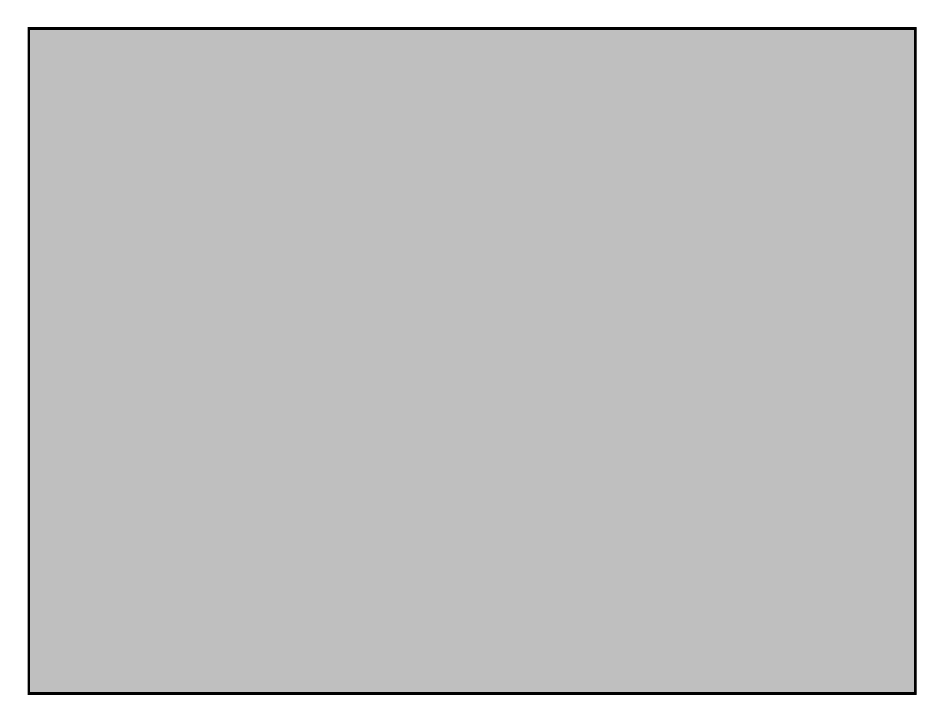
\begin{tikzpicture}[x=32bp,y=24bp]% 4x3
    \clip (0,0) rectangle (10,10);
    \path [fill=black!25] (0,0) rectangle (10,10);
    \path [draw,ultra thick] (0,0) rectangle (10,10);
\end{tikzpicture}%
%</example-image-empty.tex>
%<*example-image-empty.tex&standalone>
\end{document}%
%</example-image-empty.tex&standalone>
%<*example-image-empty.tex>
%    \end{macrocode}
